\documentclass{article}
\usepackage{graphicx}
\usepackage{amsmath, amsthm, amssymb}
\usepackage{multicol}
\usepackage[utf8]{inputenc}
\usepackage{enumerate} 
\usepackage{lmodern,microtype}
\usepackage{hyperref}
\usepackage{polski}
\usepackage{graphicx}
\usepackage{float}
\usepackage{listings}
\usepackage[a4paper, left=1.in, right=1in, top=1in, bottom=1in]{geometry}

\author{Matylda Mordal}
\title{\textbf{Lista 3 sprawozdanie}}
\date{}

\begin{document}
	\maketitle
	\section*{Zadanie 1}
		\subsection*{CUT\_ROD} 
		\begin{lstlisting}[language=C++, tabsize=3, basicstyle=\footnotesize]
int CUT_ROD(int p[], int n) {
	if (n == 0) return 0; 
	
	int q = INT_MIN;
	for (int i = 1; i <= n; ++i) { 
		q = max(q, p[i - 1] + CUT_ROD(p, n - i)); 
	}
	return q;
}
		\end{lstlisting}
	
			\subsubsection*{Działanie funkcji CUT\_ROD}
			\begin{itemize}
			\item Tablica $p[]$ zawierająca ceny prętów o różnych długościach. Liczba $n$ oznaczająca długość pręta do przecięcia.
			\item Jeśli długość pręta $n = 0$, maksymalny zysk wynosi $0$.
			\item Próbujemy podzielić pręt na dwa kawałki o długości $i$ i $n - i$ (dla każdego $i$ od 1 do $n$). \item Maksymalny zysk dla bieżącego podziału obliczamy jako $p[i - 1]$ (zysk z pręta długości $i$) + wynik rekurencji dla pozostałej długości $\texttt{CUT\_ROD}(p, n - i)$.
			\item Maksymalny zysk $q$ aktualizujemy przy każdym podziale, wybierając najlepszy możliwy podział.
			\end{itemize}
		
		\subsection*{MEMORIZED\_CUT\_ROD} 
		\begin{lstlisting}[language=C++, tabsize=3, basicstyle=\footnotesize]
int MEMORIZED_CUT_ROD(int p[], int r[], int s[], int n) {
	if (r[n] >= 0) return r[n];
	int q;
	if (n == 0) {
		q = 0; 
	} else {
		q = INT_MIN;
		for (int i = 1; i <= n; ++i) {
			int mozliwosc = p[i - 1] + MEMORIZED_CUT_ROD(p, r, s, n - i);
			if (q < mozliwosc) {
				q = mozliwosc;
				s[n] = i; 
			}
		}
	}
	r[n] = q; 
	return q;
}
	
		\end{lstlisting}
		
			\subsubsection*{Działanie funkcji MEMORIZED\_CUT\_ROD} 
			\begin{itemize} 
				\item Funkcja zapamiętuje wyniki  dla różnych długości prętów w tablicy $r[]$. 
				\item Jeśli wartość $r[n]$ jest już obliczona, funkcja zwraca zapamiętaną wartość.
				\item Jeśli długość pręta $n = 0$, maksymalny zysk wynosi $0$. 
				\item Próbujemy podzielić pręt na dwa kawałki o długości $i$ i $n - i$ (dla każdego $i$ od 1 do $n$). 
				\item Maksymalny zysk dla bieżącego podziału obliczamy jako $p[i - 1]$ (zysk z pręta długości $i$) + wynik rekurencji dla pozostałej długości $\texttt{MEMORIZED\_CUT\_ROD}(p, r, s, n - i)$.
				\item Maksymalny zysk $q$ aktualizujemy przy każdym podziale, wybierając najlepszy możliwy podział. 
				\item Wynik jest zapisywany w tablicy $r[]$. Dzięki temu późniejsze wywołania funkcji są szybsze, ponieważ można korzystać z wcześniej obliczonych wartości. \end{itemize}
			
		\subsection*{EXT\_BOT\_UP\_CUT\_ROD} 
		\begin{lstlisting}[language=C++, tabsize=3, basicstyle=\footnotesize]
int EXT_BOT_UP_CUT_ROD(int p[], int n, int r[], int s[]) {
	r[0] = 0; // Cena 0 dla 0
	for (int j = 1; j <= n; ++j) {
		int q = INT_MIN;
		for (int i = 1; i <= j; ++i) { 
			if (q < p[i - 1] + r[j - i]) {
				q = p[i - 1] + r[j - i];
				s[j] = i; 
			}
		}
		r[j] = q; 
	}
	return r[n];
}
				
		\end{lstlisting}
		
			\subsubsection*{Działanie funkcji EXT\_BOT\_UP\_CUT\_ROD} 
			\begin{itemize}
				\item Funkcja rozpoczyna od przypisania zera dla długości pręta $r[0]$.
				\item Dla każdej długości pręta $j$ od 1 do $n$:
				\begin{itemize}
					\item Funkcja sprawdza wszystkie możliwe podziały pręta na kawałki o długości $i$ i $j - i$.
					\item Maksymalny zysk $q$ jest aktualizowany jako suma zysku z kawałka o długości $i$ ($p[i - 1]$) oraz wyniku dla pozostałej długości ($r[j - i]$).
					\item Zapamiętuje optymalną długość cięcia w tablicy $s[]$.
				\end{itemize}
				\item Wynik: Funkcja zwraca wartość $r[n]$, czyli maksymalny zysk dla długości pręta $n$.
			\end{itemize}
		
	\newpage
	\section*{Zadanie 2}
	\begin{figure}[H]
		\centering
		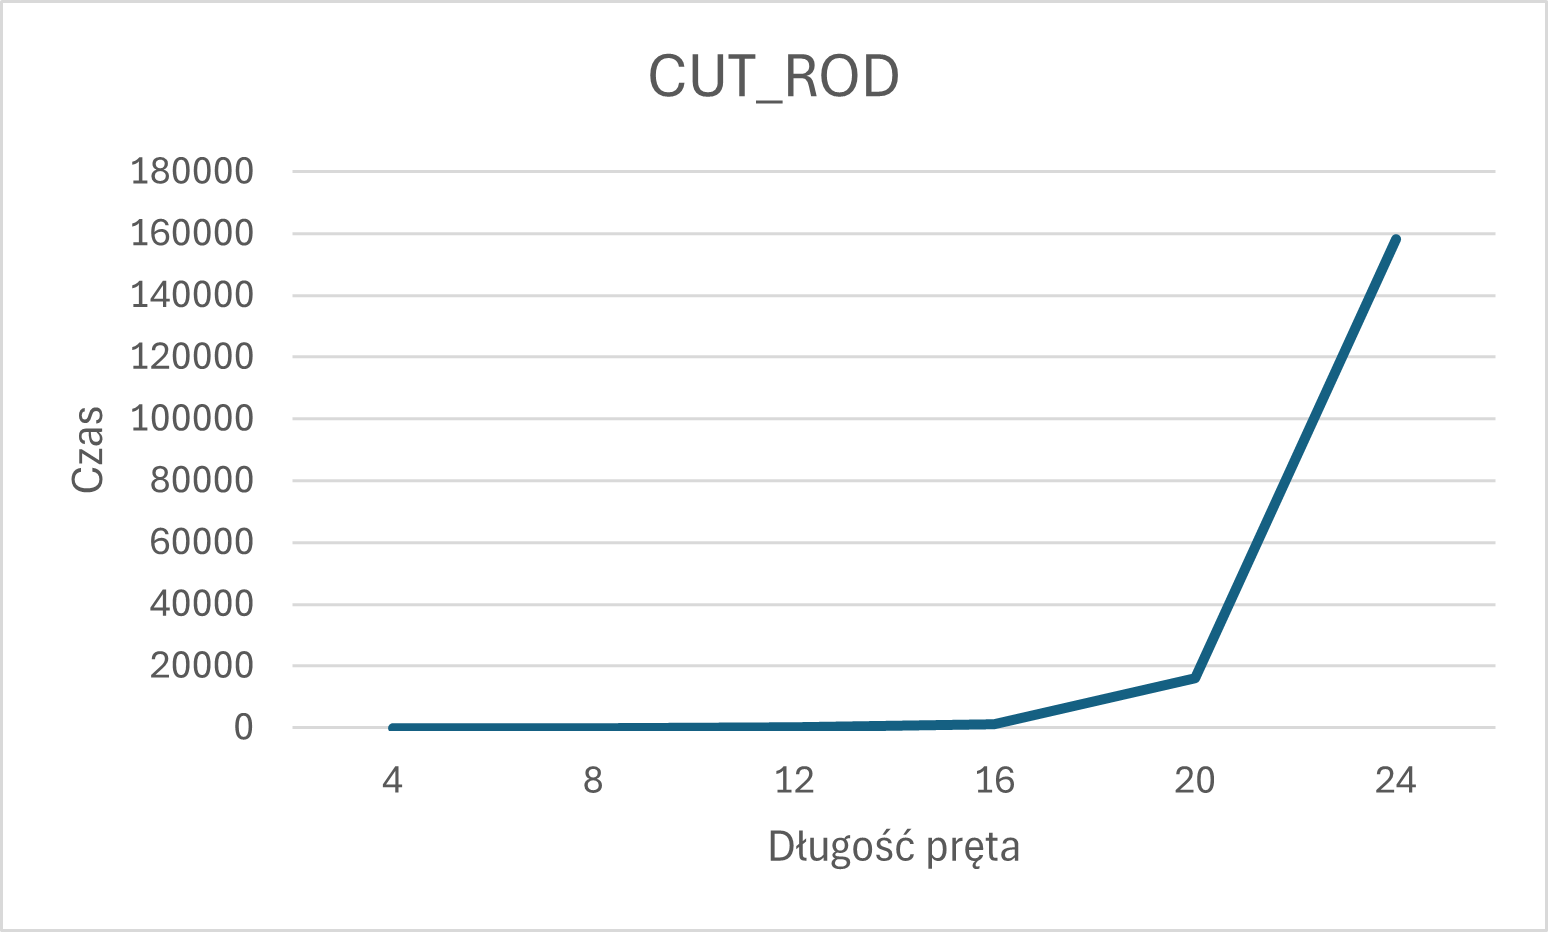
\includegraphics[width=0.9\textwidth]{CutRod.png}
	\end{figure}
	
	\subsection*{Wnioski} 
	
Algorytm rekurencyjny CUT\_ROD wykonuje ogromną liczbę operacji, która rośnie bardzo szybko wraz z długością pręta, zgodnie z wykładniczą złożonością czasową \( O(2^n) \). Przykładowo, dla długości 16 wykonuje 1251 operacji, a dla długości 24 już 158163. Ponieważ algorytm nie zapamiętuje wcześniej obliczonych wyników, wielokrotnie przelicza te same wartości, co powoduje gwałtowny wzrost liczby operacji. Wykres przybiera charakterystyczny kształt krzywej wykładniczej, gwałtownie rosnącej wraz z długością pręta.
	
	\begin{figure}[H]
		\begin{minipage}{0.5\textwidth}
			\centering
			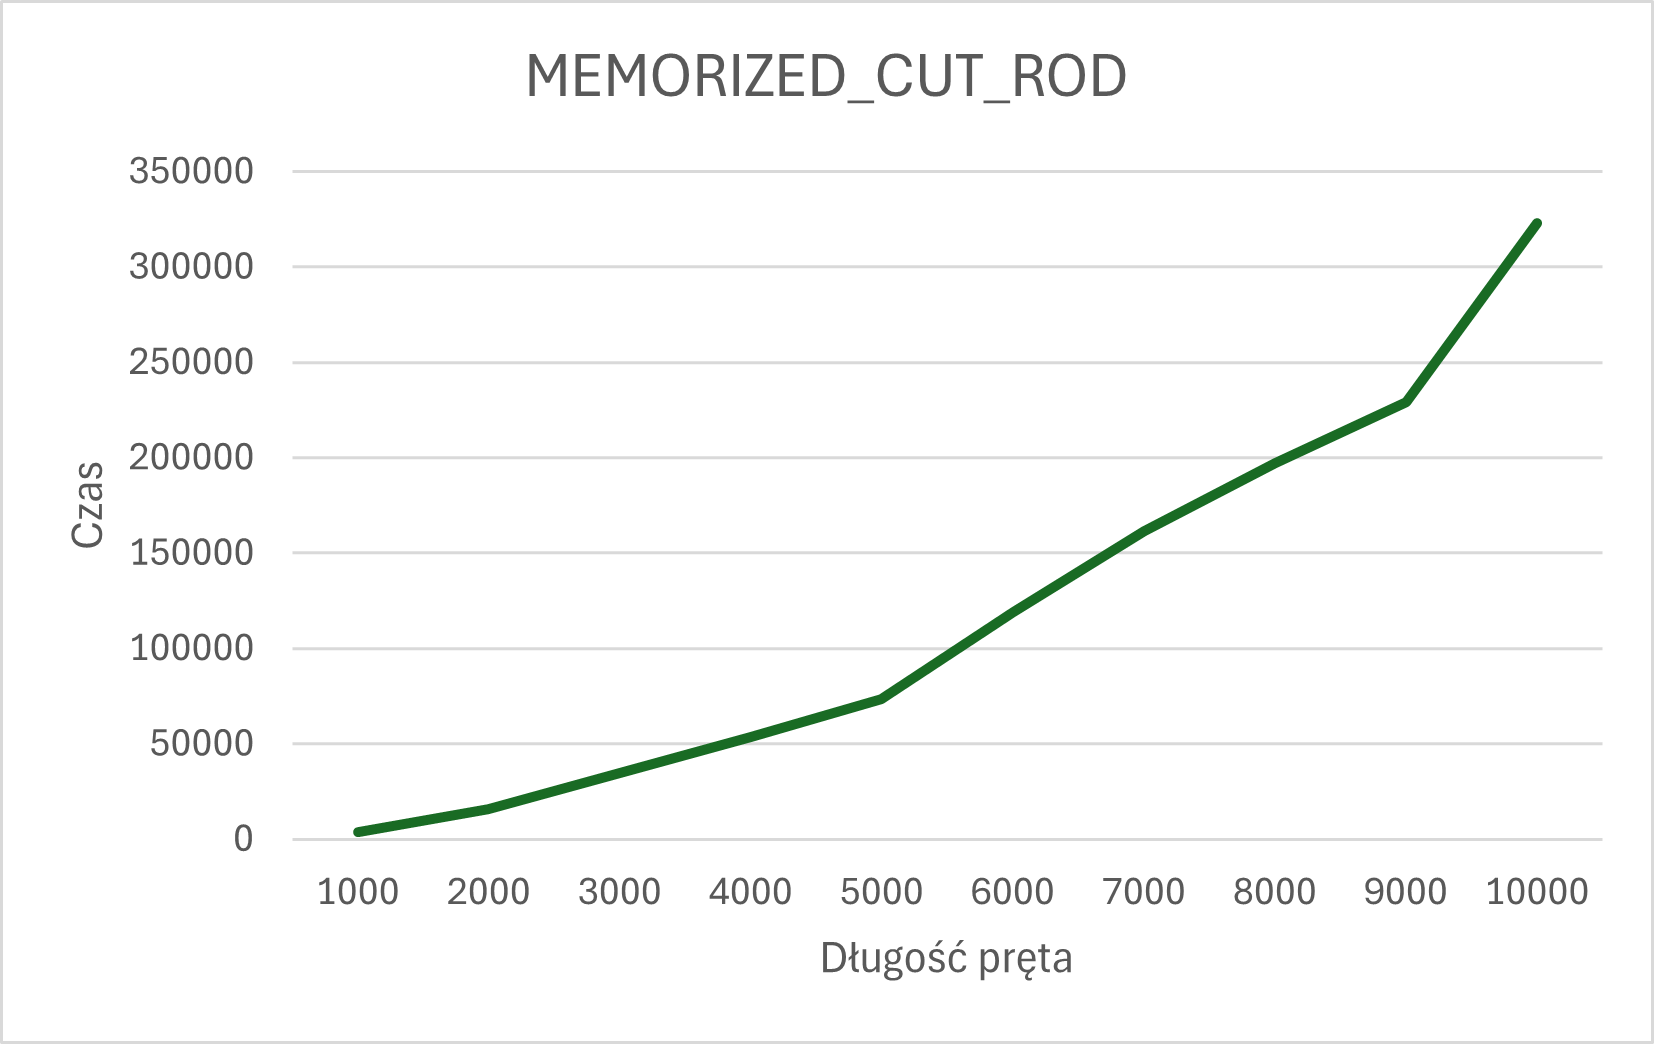
\includegraphics[width=\textwidth]{MemoCR.png}
		\end{minipage}%
		\begin{minipage}{0.5\textwidth}
			\centering
			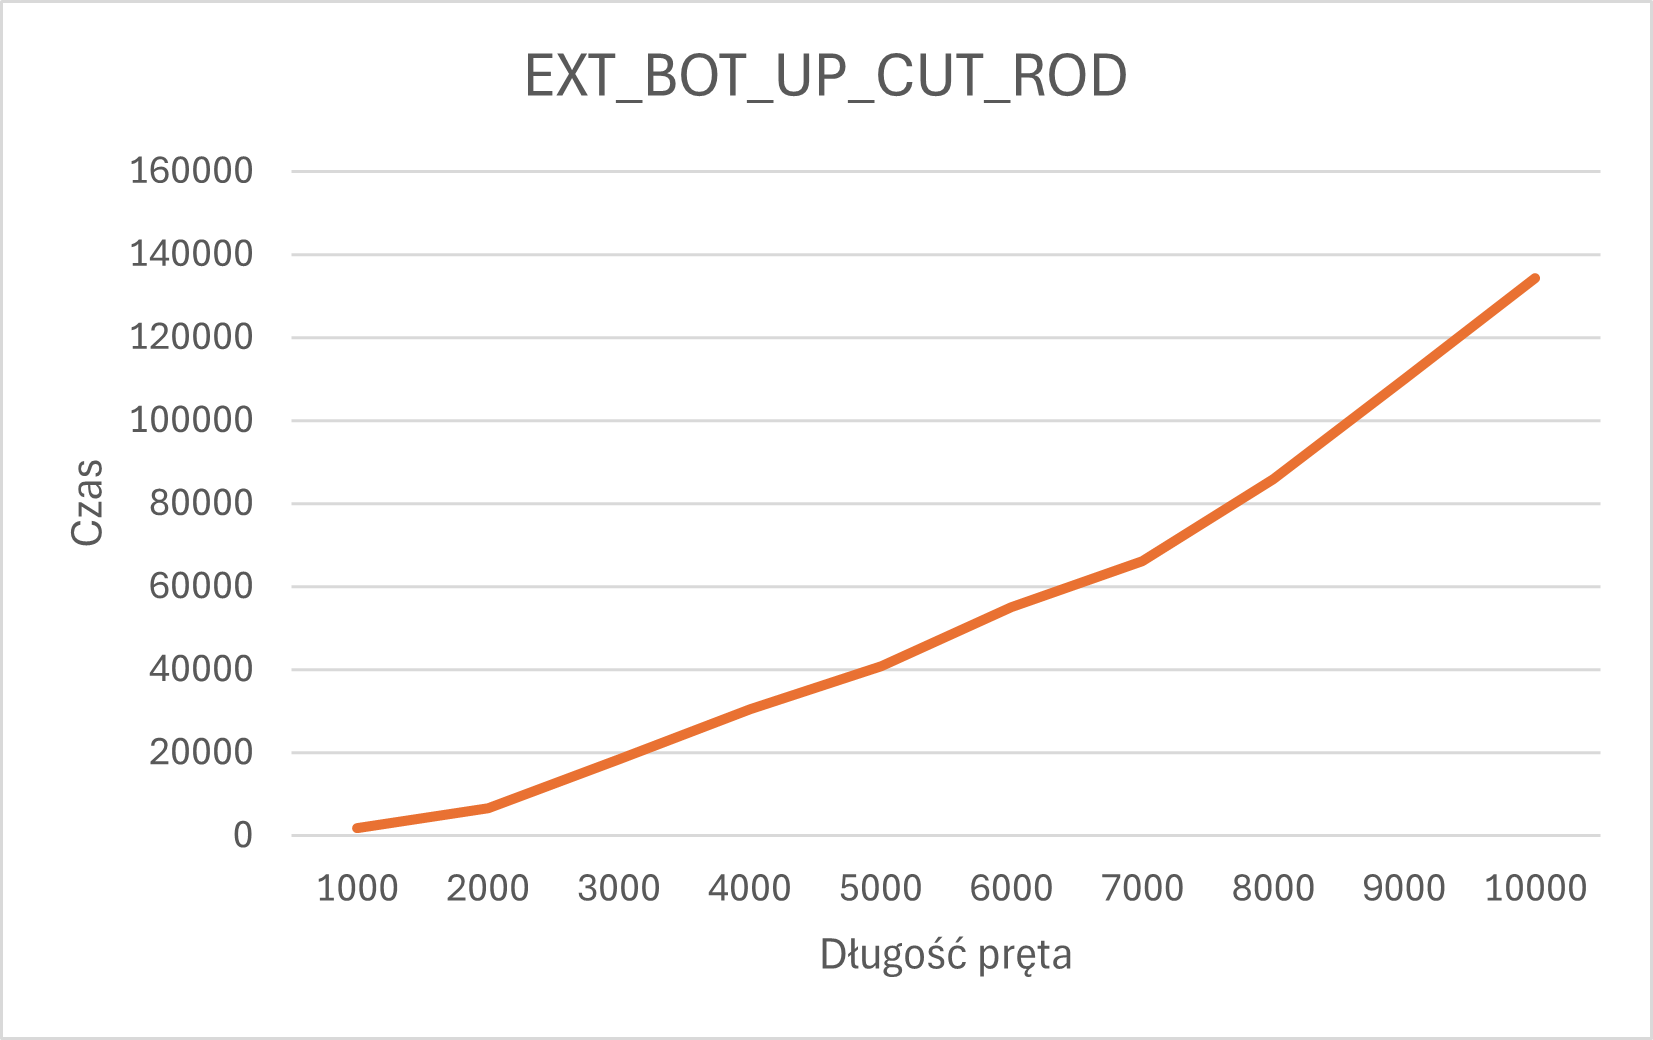
\includegraphics[width=\textwidth]{ExtCR.png}
		\end{minipage}
	\end{figure}
	
	\subsection*{Wnioski} 
	Algorytm MEMORIZED\_CUT\_ROD oparty na memoizacji ma złożoność $O(n^2)$. Dzięki eliminacji nadmiarowych obliczeń działa szybciej niż standardowy algorytm rekurencyjny, ale przy dużych długościach pręta jego czas działania nadal znacząco rośnie. 
	Algorytm EXT\_BOT\_UP\_CUT\_ROD również ma złożoność $O(n^2)$, ale działa iteracyjnie, co czyni go bardziej wydajnym. Podejście zastosowane w tym kodzie redukuje koszty zarządzania pamięcią i narzut rekurencji, przez co osiąga lepsze wyniki dla dużych danych.
	
	\begin{figure}[H]
		\begin{minipage}{0.465\textwidth}
			\centering
			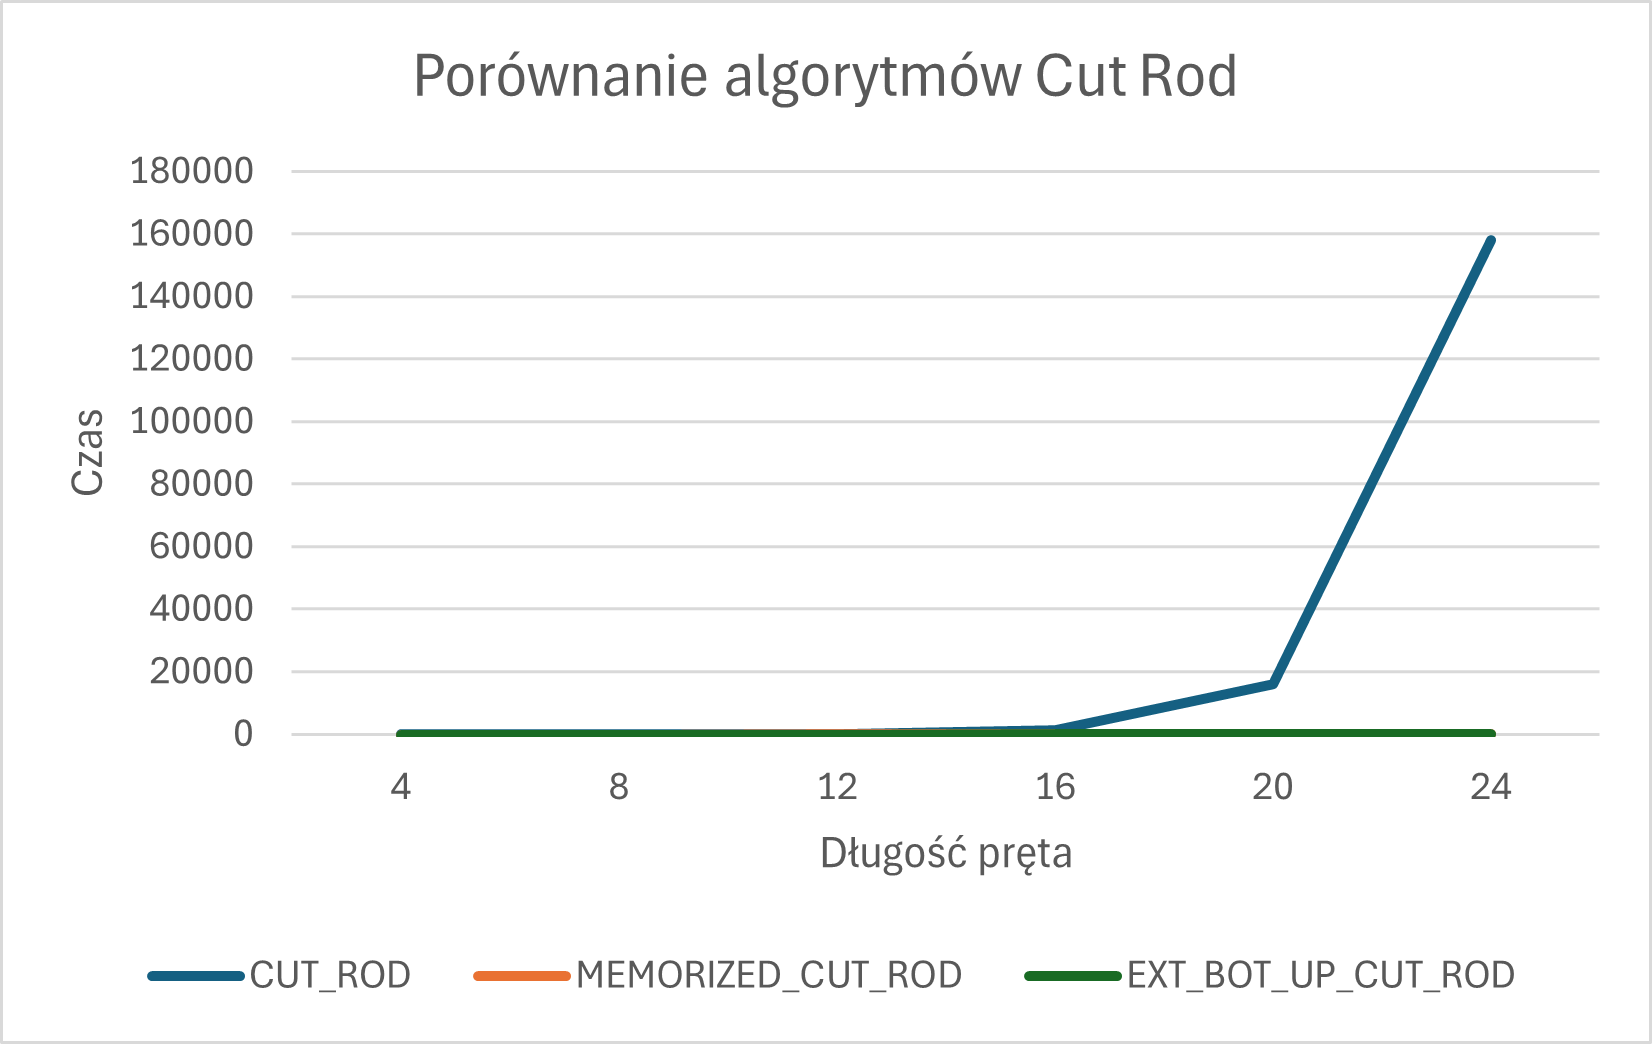
\includegraphics[width=\textwidth]{PorCR.png}
		\end{minipage}%
		\begin{minipage}{0.535\textwidth}
			\centering
			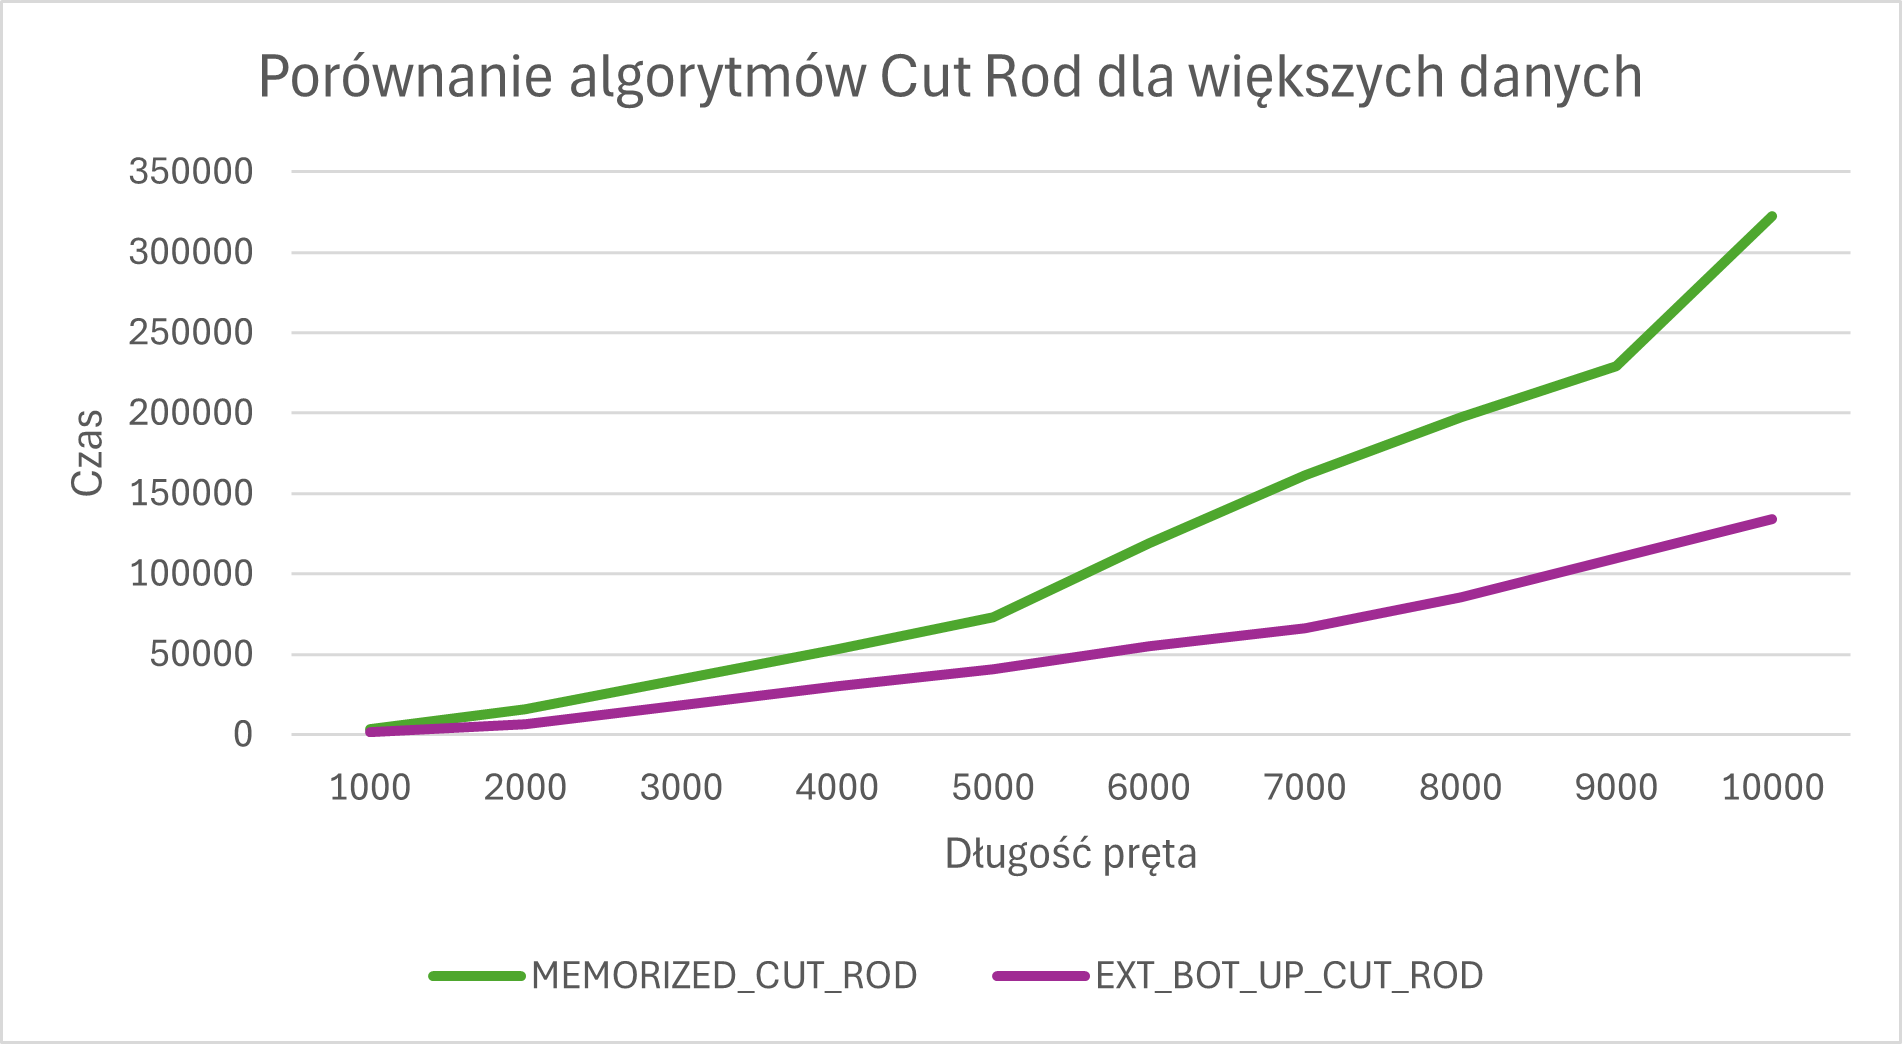
\includegraphics[width=\textwidth]{PorCR2.png}
		\end{minipage}
	\end{figure}
	
	\subsection*{Wnioski} 
	CUT\_ROD jest zdecydowanie najmniej wydajnym rozwiązaniem, co doskonale widać na wykresie. W porównaniu do MEMORIZED\_CUT\_ROD i EXT\_BOT\_UP\_CUT\_ROD, które wykazują znacznie większą efektywność już przy mniejszych zbiorach danych.
	Natomiast z drugiego wykresu widać, że wraz ze wzrostem długości pręta, zarówno wartość MEMORIZED\_CUT\_ROD, jak i EXT\_BOT\_UP\_CUT\_ROD rosną w sposób wykładniczy. Dla każdej długości pręta wartości te znacząco się różnią, z wyraźnie wyższymi wartościami dla MEMORIZED\_CUT\_ROD. 
	
	
	\newpage
	\section*{Zadanie 3}
	\subsection*{LCS\_REKU\_SPAM} 
	\begin{lstlisting}[language=C++, tabsize=2, basicstyle=\footnotesize]
int LCS_REKU_SPAM(const string &s1, const string &s2, int m, int n, int **b) { 
	if (m == 0 || n == 0) 
	return 0;
	
	if (b[m][n] != -1) 
	return b[m][n];
	
	if (s1[m - 1] == s2[n - 1]) 
	return b[m][n] = 1 + LCS_REKU_SPAM(s1, s2, m - 1, n - 1, b);

	b[m][n] = max(LCS_REKU_SPAM(s1, s2, m, n - 1, b), LCS_REKU_SPAM(s1, s2, m - 1, n, b));
	return b[m][n] ;
}
		
	\end{lstlisting}
	
		\subsubsection*{Działanie funkcji LCS\_REKU\_SPAM}
		\begin{itemize}
			\item Jeśli $m$ lub $n$ wynosi $0$ (czyli dotarliśmy do początku jednego z napisów), zwracane jest $0$, ponieważ nie ma już żadnych znaków do porównania.
			\item Jeśli wartość $b[m][n]$ jest różna od $-1$, oznacza to, że wynik dla tej pary indeksów został już obliczony wcześniej. W takim przypadku zwracana jest zapisana wartość.
			\item Jeśli znak $s1[m-1]$ jest równy $s2[n-1]$, oznacza to, że znak ten należy do szukanego podciągu.
			\item Wywoływana jest funkcja rekurencyjnie z indeksami $m-1$ i $n-1$, a wynik jest zwiększany o $1$ i zapisywany w $b[m][n]$.
			\item Jeśli ostatnie znaki nie są równe, funkcja wybiera maksymalny wynik z dwóch możliwych ścieżek:
			\begin{itemize}
				\item Pominięcie ostatniego znaku $s2$ ($m, n-1$).
				\item Pominięcie ostatniego znaku $s1$ ($m-1, n$).
			\end{itemize}
			\item Wynik maksymalny jest zapisywany w $b[m][n]$.
			\item Funkcja zwraca wartość $b[m][n]$, czyli maksymalną długość podciągu.
		\end{itemize}

	\subsection*{LCS\_ITERA} 
	\begin{lstlisting}[language=C++, tabsize=3, basicstyle=\footnotesize]
char** LCS_ITERA(string& s1, string& s2, int& dlugosc) {
	int m = s1.length();
	int n = s2.length();
	
	int** c = new int*[m + 1];
	char** b = new char*[m + 1];
	for (int i = 0; i <= m; i++) {
		c[i] = new int[n + 1];
		b[i] = new char[n + 1];
	}
	
	for (int i = 0; i <= m; i++) c[i][0] = 0;
	for (int j = 0; j <= n; j++) c[0][j] = 0;
	
	for (int i = 1; i <= m; i++) {
		for (int j = 1; j <= n; j++) {
			if (s1[i - 1] == s2[j - 1]) {
				c[i][j] = c[i - 1][j - 1] + 1;
				b[i][j] = '\\'; 
			} else if (c[i - 1][j] >= c[i][j - 1]) {
				c[i][j] = c[i - 1][j];
				b[i][j] = '|'; 
			} else {
				c[i][j] = c[i][j - 1];
				b[i][j] = '-'; 
			}
		}
	}
	
	dlugosc = c[m][n];
	
	for (int i = 0; i <= m; i++) {
		delete[] c[i];
	}
	delete[] c;
	
	return b;
}
		
	\end{lstlisting}
		
		\subsubsection*{Działanie funkcji LCS\_ITERA}
		\begin{itemize}
			\item Funkcja przyjmuje dwa napisy $s1$ i $s2$ oraz referencję do zmiennej długosc.
			\item Na początku obliczane są długości napisów $m$ i $n$.
			\item Tworzone są dwie tablice dynamiczne: 
			\begin{itemize} 
				\item Tablica $c$ o wymiarach $(m+1) \times (n+1)$ przechowująca długości LCS dla odpowiednich podciągów. 
				\item Tablica $b$ o wymiarach $(m+1) \times (n+1)$ przechowująca kierunki, które pozwalają odtworzyć LCS.
			\end{itemize}
			\item Następnie wiersz i kolumna zerowa w tablicy $c$ są wypełniane zerami, ponieważ dla pustego napisu długość LCS wynosi $0$. 
			\item Algorytm dynamiczny wypełnia tablice $c$ i $b$: 
			\begin{itemize}
				\item Iteracja rozpoczyna się od $i = 1$ i $j = 1$.
				\item Jeśli znak $s1[i-1]$ jest równy $s2[j-1]$, oznacza to, że znak należy do LCS. Tablica $c[i][j]$ jest obliczana jako $c[i-1][j-1] + 1$, a w tablicy $b[i][j]$ zapisywany jest znak '\textbackslash' oznaczający ruch diagonalny.
				\item Jeśli znaki są różne, wybierana jest maksymalna wartość między $c[i-1][j]$ (pominięcie znaku w $s1$) oraz $c[i][j-1]$ (pominięcie znaku w $s2$). Kierunek ruchu jest odpowiednio oznaczany jako `\textbar` (w górę) lub '-' (w lewo).
			\end{itemize}
			\item Po zakończeniu iteracji długość LCS jest zapisana w $c[m][n]$ i przekazywana przez referencję w zmiennej długośsc.
			\item Tablica $c$ jest zwalniana z pamięci, a tablica $b$ jest zwracana jako wynik funkcji.
		\end{itemize}

	\newpage
	\section*{Zadanie 4}
	
	\begin{figure}[H]
		\begin{minipage}{0.5\textwidth}
			\centering
			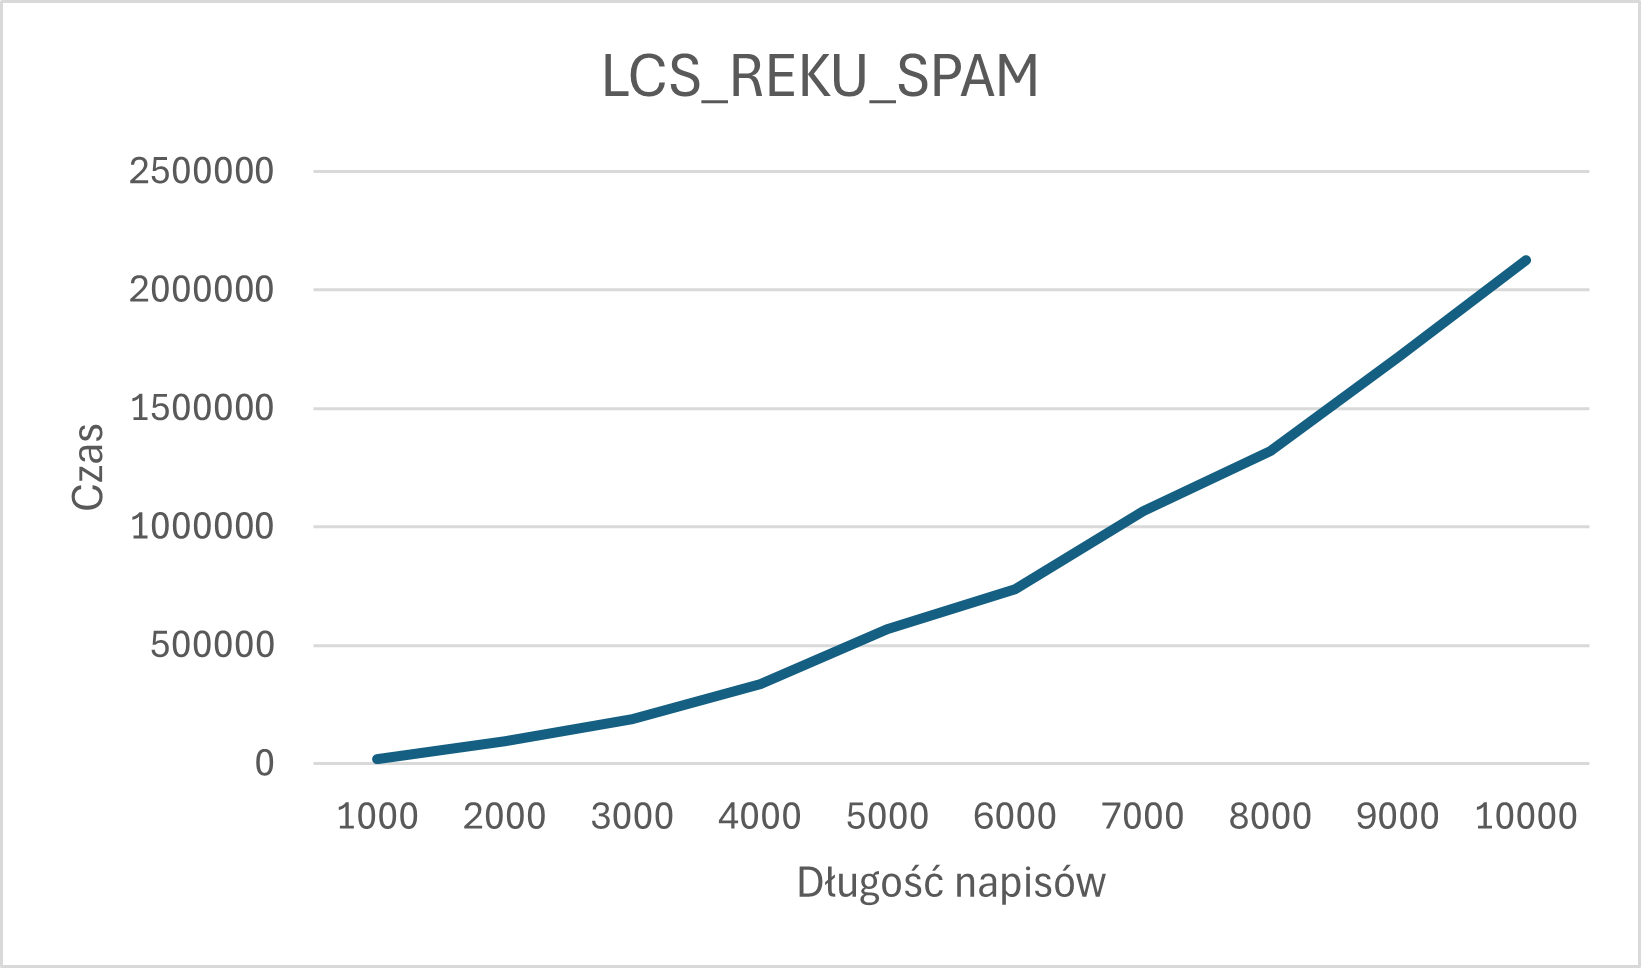
\includegraphics[width=\textwidth]{RekuLSC.png}
		\end{minipage}%
		\begin{minipage}{0.5\textwidth}
			\centering
			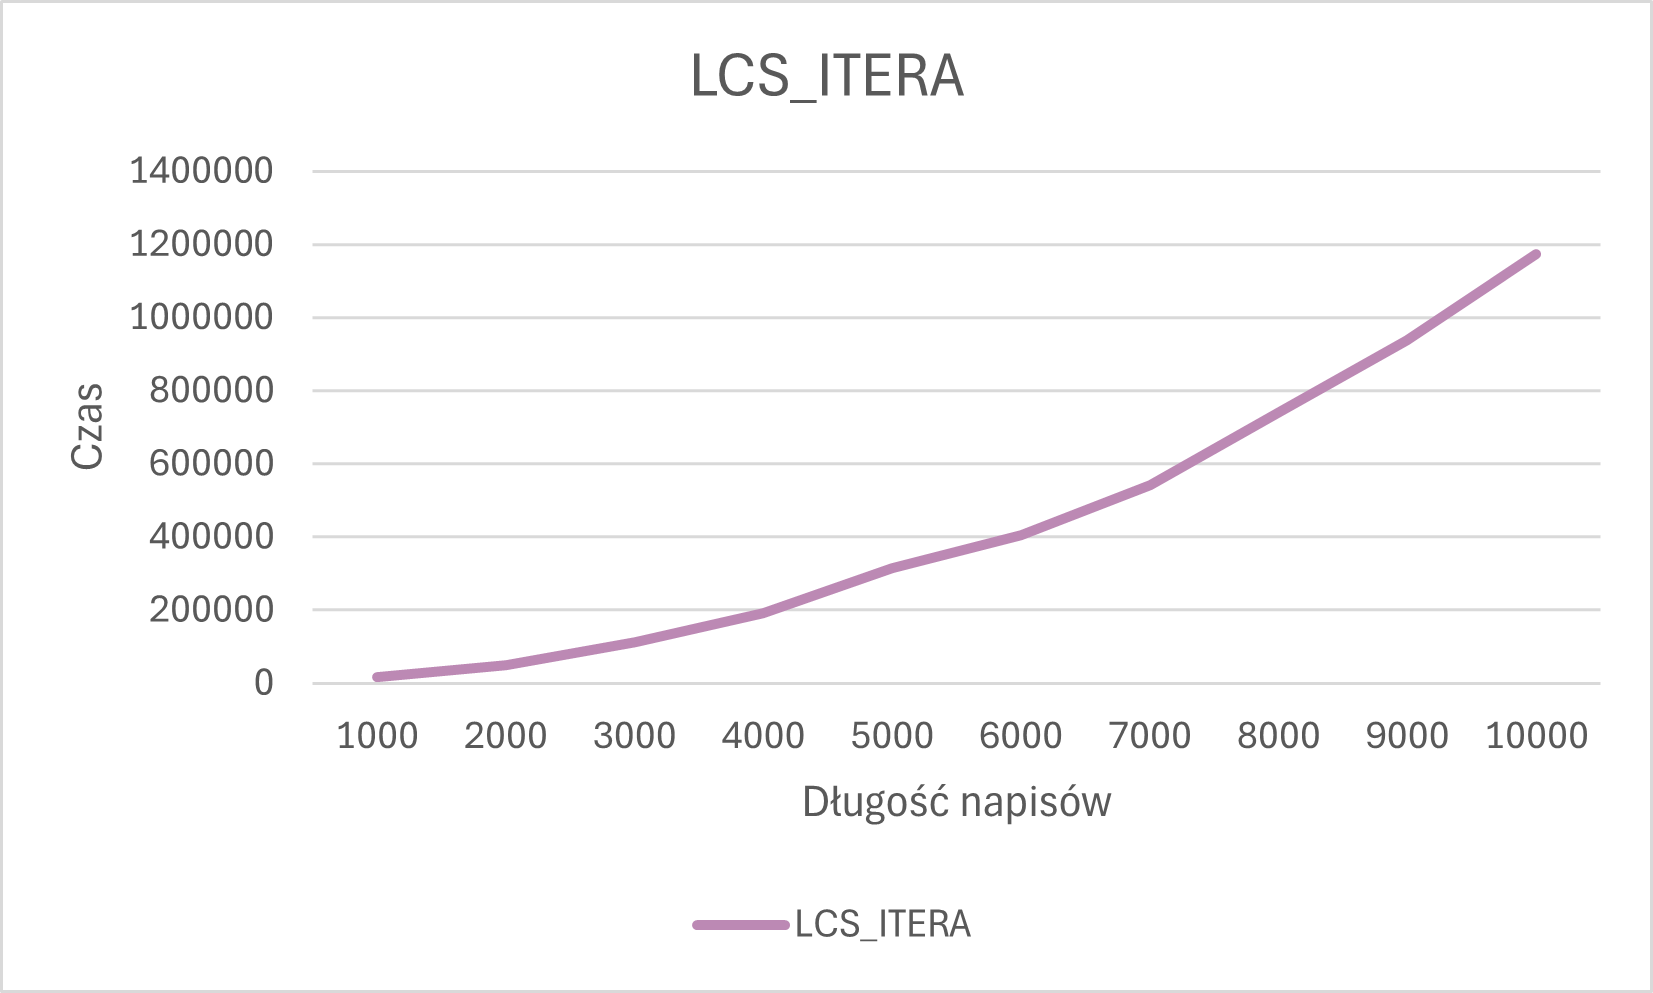
\includegraphics[width=\textwidth]{IteLSC.png}
		\end{minipage}
	\end{figure}
	
	\subsection*{Wnioski} 
	Algorytm LCS\_REKU\_SPAM charakteryzuje się wysokimi czasami wykonania, które rosną bardzo szybko wraz ze wzrostem długości napisów. Jest to związane z jego wykładniczą złożonością czasową $O(2^n)$, co wynika z jego rekurencyjnej natury. Algorytm LCS\_ITERA osiąga lepsze czasy wykonania, ponieważ wykorzystuje podejście iteracyjne z tablicą dynamiczną. Jego złożoność czasowa to $O(n*m)$, gdzie $n$ i $m$ to długości dwóch porównywanych napisów. Dzięki temu algorytm jest efektywniejszy przy większych danych wejściowych.
	
	\begin{figure}[H]
		\centering
		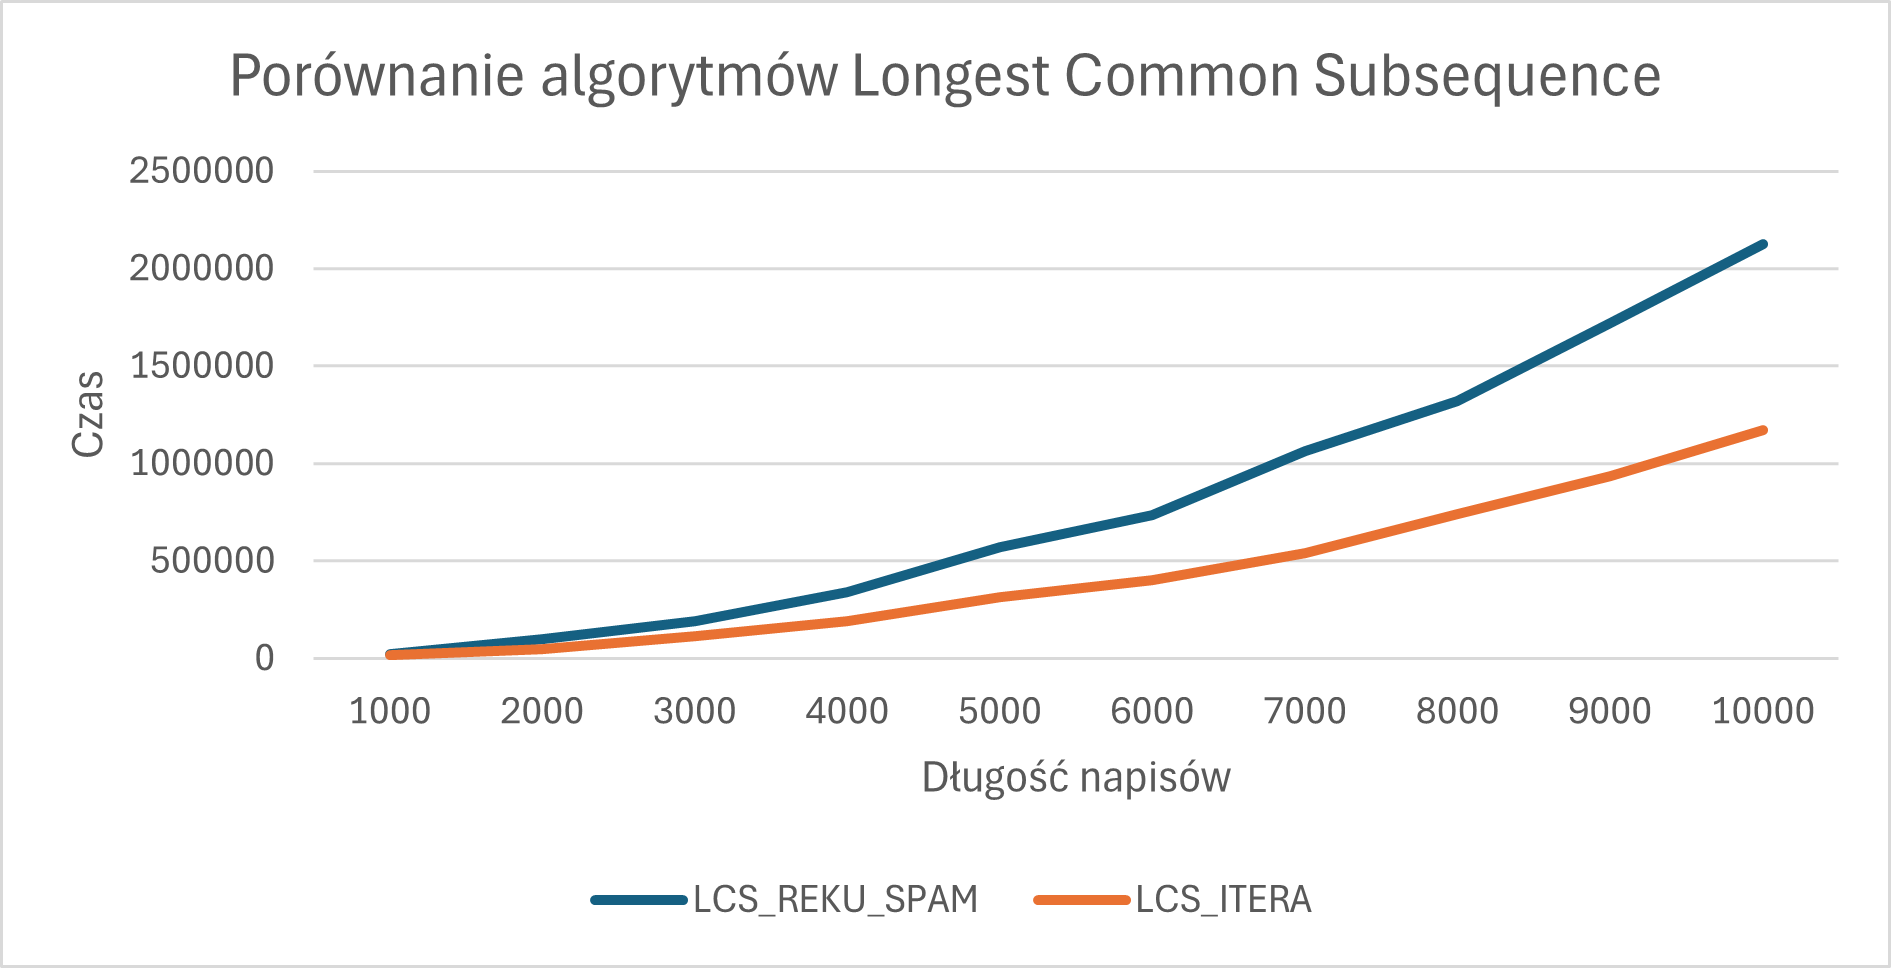
\includegraphics[width=0.9\textwidth]{PorLSC.png}
	\end{figure}
	
	\subsection*{Wnioski} 
	Algorytm LCS\_REKU\_SPAM jest mniej wydajny od LCS\_ITERA ze względu na swoją wykładniczą złożoność, podczas gdy LCS\_ITERA, działa szybciej i lepiej skaluje się dla dłuższych napisów.
	
	\newpage
	\section*{Zadanie 5}
	\subsection*{RECURSIVE\_ACTIVITY\_SELECTOR} 
	\begin{lstlisting}[language=C++, tabsize=3, basicstyle=\footnotesize]
void RECURSIVE_ACTIVITY_SELECTOR(int s[], int f[], int n, int k, int zajecia[], int &ile) {
	int m = k + 1;
	while (m <= n && s[m] < f[k]) { 
		m++;
	}
	if (m <= n) {
		zajecia[ile++] = m; 
		RECURSIVE_ACTIVITY_SELECTOR(s, f, n, m, zajecia, ile);  
	}
}

		
	\end{lstlisting}
	
		\subsubsection*{Działanie funkcji RECURSIVE\_ACTIVITY\_SELECTOR}
		\begin{itemize}
			\item \textbf{Parametry :}
			\begin{itemize}
				\item $s[]$ - tablica czasów rozpoczęcia zajęć
				\item $f[]$ - tablica czasów zakończenia zajęć, uporządkowana rosnąco.
				\item $n$ - liczba zajęć (indeks ostatniego elementu w $s[]$ i $f[]$).
				\item $k$ - indeks ostatnio wybranego zajęcia.
				\item $result[]$ - tablica wynikowa, w której przechowywane są indeksy wybranych zajęć.
				\item $count$ - liczba wybranych zajęć .
			\end{itemize}
			\item \textbf{Działanie:}
			\begin{itemize}
				\item Chcemy znaleźć zbiór zajęć, które nie nachodzą na siebie, zaczynając od działania o indeksie $k$.
				\item  Funkcja zaczyna od zajęcia o indeksie $k$ i szuka pierwszego zajęcia $m$, które nie koliduje z wybranym zajęciem $k$. Czas rozpoczęcia $s[m]$ musi być większy lub równy czasowi zakończenia $f[k]$.
				\item  Funkcja porusza się przez tablicę, zwiększając $m$, dopóki nie znajdzie pierwszego zajęcia, które spełnia powyższy warunek.
				\item Po znalezieniu takiego zajęcia:
				\begin{itemize}
					\item Dodaje jego indeks do $result[]$.
					\item Zwiększa licznik $count$.
					\item Wywołuje się ponownie dla zajęcia $m$ jako nowego ostatniego wybranego zajęcia.
				\end{itemize}
				\item Rekurencja kończy się, gdy $m > n$. 
			\end{itemize}
		
		\end{itemize}
		
	\subsection*{ACTIVITY\_SELECTOR} 
	\begin{lstlisting}[language=C++, tabsize=3, basicstyle=\footnotesize]
void ACTIVITY_SELECTOR(int s[], int f[], int n, int zajecia[], int &ile){
	zajecia[ile++] = 1; 
	int k = 1;
	
	for (int m = 2; m <= n; m++) {
		if (s[m] >= f[k]) {
			zajecia[ile++] = m; 
			k = m;
		}
	}
}
	\end{lstlisting}

		\subsubsection*{Działanie funkcji ACTIVITY\_SELECTOR}
		\begin{itemize}
			\item Tablica $result[]$, która przechowuje indeksy wybranych zajęć.
			\item Zmienna $count$ służy do liczenia liczby wybranych zajęć.
			\item Pierwsza aktywność (o indeksie $1$) jest zawsze wybierana. 
			\item Indeks $k$ przechowuje indeks ostatnio wybranego zajęcia (na początku $1$).
			\item Pętla iteruje przez kolejne zajęcia (od $m = 2$ do $m = n$).
			\item Sprawdzane jest, czy czas rozpoczęcia zajęcia $s[m]$ jest większy lub równy czasowi zakończenia ostatniego wybranego zajęcia $f[k]$.
			\item Jeśli warunek jest spełniony:
			\begin{itemize}
				\item Indeks $m$ zostaje dodany do tablicy $result[]$.
				\item Zmienna $count$ jest zwiększana.
				\item Zmienna $k$ jest aktualizowana na $m$ (ostatnio wybrane zajęcie).
			\end{itemize}
			\item Pętla kończy działanie po przetworzeniu wszystkich zajęć ($m > n$)
		\end{itemize}
		
	\subsection*{RECURSIVE\_ACTIVITY\_SELECTOR2} 
\begin{lstlisting}[language=C++, tabsize=3, basicstyle=\footnotesize]
void RECURSIVE_ACTIVITY_SELECTOR2(int s[], int f[], int k, int zajecia[], int &ile) {
	int m = k - 1;
	while (m > 0 && f[m] > s[k]) {
		m--;
	}
	if (m > 0) { 
		zajecia[ile++] = m; 
		RECURSIVE_ACTIVITY_SELECTOR2(s, f, m, zajecia, ile);  
	}
}
	
\end{lstlisting}
		
		\subsubsection*{Działanie funkcji RECURSIVE\_ACTIVITY\_SELECTOR2}
		\begin{itemize}
			\item Funkcja rekurencyjnie wybiera zajęcia, zaczynając od zadanego indeksu $k$.
			\item Indeks $m$ przechowuje potencjalny indeks zajęcia, które kończy się przed rozpoczęciem zajęcia o indeksie $k$.
			\item Pętla \texttt{while} iteruje wstecz przez indeksy zajęć (od $m = k-1$ do $m > 0$):
			\begin{itemize}
				\item Sprawdzane jest, czy czas zakończenia zajęcia $f[m]$ jest mniejszy lub równy czasowi rozpoczęcia zajęcia $s[k]$.
				\item Pętla kończy działanie, gdy znajdzie takie zajęcie lub gdy $m = 0$.
			\end{itemize}
			\item Jeśli znaleziono pasujące zajęcie ($m > 0$):
			\begin{itemize}
				\item Indeks $m$ zostaje dodany do tablicy $zajecia[]$.
				\item Zmienna $ile$ jest zwiększana.
				\item Funkcja wywołuje samą siebie rekurencyjnie z parametrami $s$, $f$, $m$, $zajecia$ oraz $ile$.
			\end{itemize}
			\item Rekurencja kończy działanie, gdy nie ma już pasujących zajęć ($m \leq 0$).
			\item Po zakończeniu rekurencji tablica $zajecia[]$ zawiera indeksy wybranych zajęć w kolejności od najpóźniejszego do najwcześniejszego.
		\end{itemize}

	\subsection*{ACTIVITY\_SELECTOR2} 
\begin{lstlisting}[language=C++, tabsize=3, basicstyle=\footnotesize]
void ACTIVITY_SELECTOR2(int s[], int f[], int n, int zajecia[], int &ile) {
	zajecia[ile++] = n - 1; 
	int k = n - 1;
	
	for (int m = n - 2; m >= 1; m--) {
		if (f[m] <= s[k]) {
			zajecia[ile++] = m; 
			k = m;
		}
	}
}
\end{lstlisting}
		
		\subsubsection*{Działanie funkcji ACTIVITY\_SELECTOR2}
		\begin{itemize}
			\item Ostatnie zajęcie (o indeksie $n-1$) jest zawsze wybierane jako pierwsze.
			\item Indeks $k$ przechowuje indeks ostatnio wybranego zajęcia (początkowo $n-1$).
			\item Pętla iteruje wstecz przez kolejne zajęcia (od $m = n-2$ do $m = 1$):
			\begin{itemize}
				\item Sprawdzane jest, czy czas zakończenia zajęcia $f[m]$ jest mniejszy lub równy czasowi rozpoczęcia ostatnio wybranego zajęcia $s[k]$.
				\item Jeśli warunek jest spełniony:
				\begin{itemize}
					\item Indeks $m$ zostaje dodany do tablicy $zajecia[]$.
					\item Zmienna $ile$ jest zwiększana.
					\item Zmienna $k$ jest aktualizowana na $m$.
				\end{itemize}
			\end{itemize}
			\item Pętla kończy działanie po przeanalizowaniu wszystkich zajęć ($m < 1$).
			\item Po zakończeniu działania tablica $zajecia[]$ zawiera indeksy wybranych zajęć w kolejności od najpóźniejszego do najwcześniejszego.
		\end{itemize}
	
	\subsection*{DYNAMIC\_ACTIVITY\_SELECTOR} 
	\begin{lstlisting}[language=C++, tabsize=3, basicstyle=\footnotesize]
void DYNAMIC_ACTIVITY_SELECTOR(int s[], int f[], int n) {
	int **c = new int *[n + 2];
	int **b = new int *[n + 2];
	for (int i = 0; i < n + 2; ++i) {
		c[i] = new int[n + 2]{0};
		b[i] = new int[n + 2]{0};
	}
	
	for (int i = 0; i <= n; ++i) {
		c[i][i] = 0;
		c[i][i + 1] = 0;
	}
	c[n + 1][n + 1] = 0;
	
	for (int l = 2; l <= n + 1; ++l) {
		for (int i = 0; i <= n - l + 1; ++i) {
			int j = i + l;
			c[i][j] = 0;
			for (int k = j - 1; k > i; --k) {
				if (f[i] <= s[k] && f[k] <= s[j] && c[i][k] + c[k][j] + 1 > c[i][j]) {
					c[i][j] = c[i][k] + c[k][j] + 1;
					b[i][j] = k;
				}
			}
		}
	}
	
	for (int i = 0; i < n + 2; ++i) {
		delete[] c[i];
		delete[] b[i];
	}
	delete[] c;
	delete[] b;
}

	\end{lstlisting}
		
		\subsubsection*{Działanie funkcji DYNAMIC\_ACTIVITY\_SELECTOR}
		\begin{itemize}
			\item Funkcja wykorzystuje dynamiczne programowanie do wybrania maksymalnej liczby zajęć, które nie nakładają się czasowo.
			\item Tworzone są dwie tablice: 
			\begin{itemize}
				\item Tablica $c[i][j]$ przechowuje maksymalną liczbę aktywności w przedziale od $i$ do $j$.
				\item Tablica $b[i][j]$ przechowuje indeks ostatnio wybranej aktywności w tym przedziale.
			\end{itemize}
			\item Dla każdego możliwego przedziału długości od 2 do $n+1$, funkcja iteruje przez wszystkie możliwe aktywności i aktualizuje tablicę $c[i][j]$ na podstawie warunku, że aktywność $k$ może być wybrana.
			\item Funkcja kończy po obliczeniu maksymalnej liczby aktywności dla wszystkich przedziałów.
		\end{itemize}
	\newpage
	\section*{Zadanie 6}
	
		\begin{figure}[H]
		\begin{minipage}{0.5\textwidth}
			\centering
			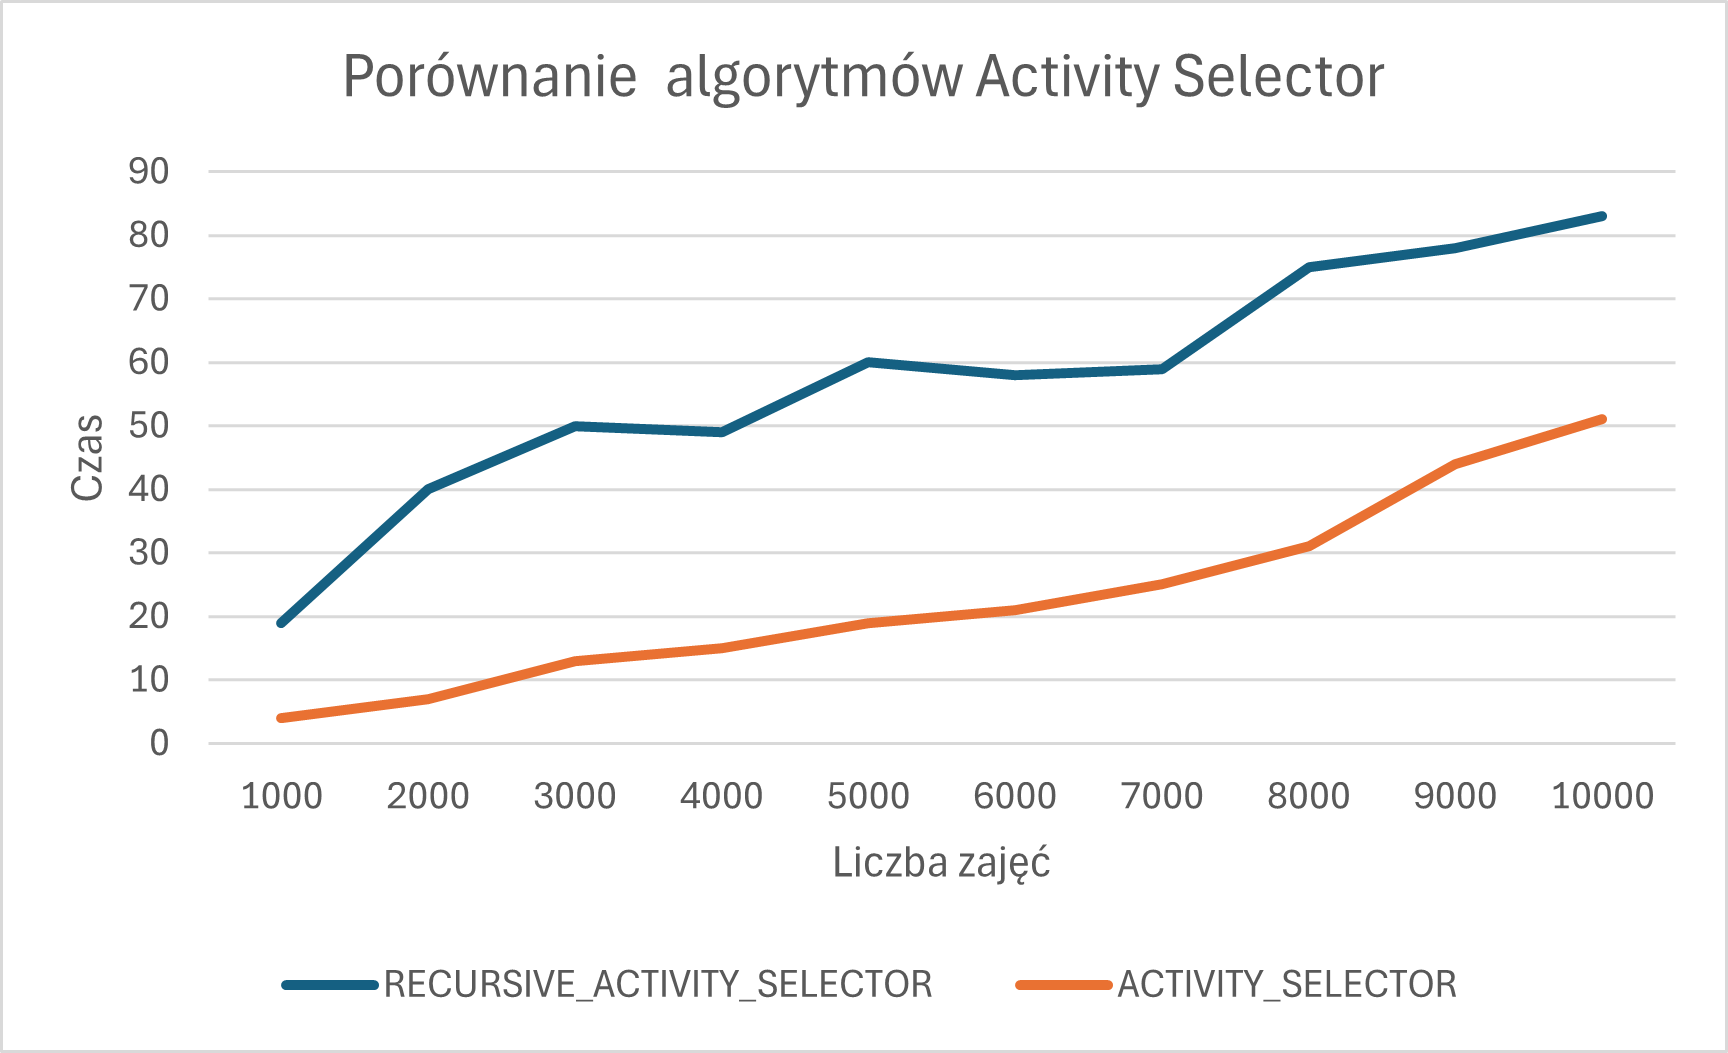
\includegraphics[width=\textwidth]{AS1.png}
		\end{minipage}%
		\begin{minipage}{0.5\textwidth}
			\centering
			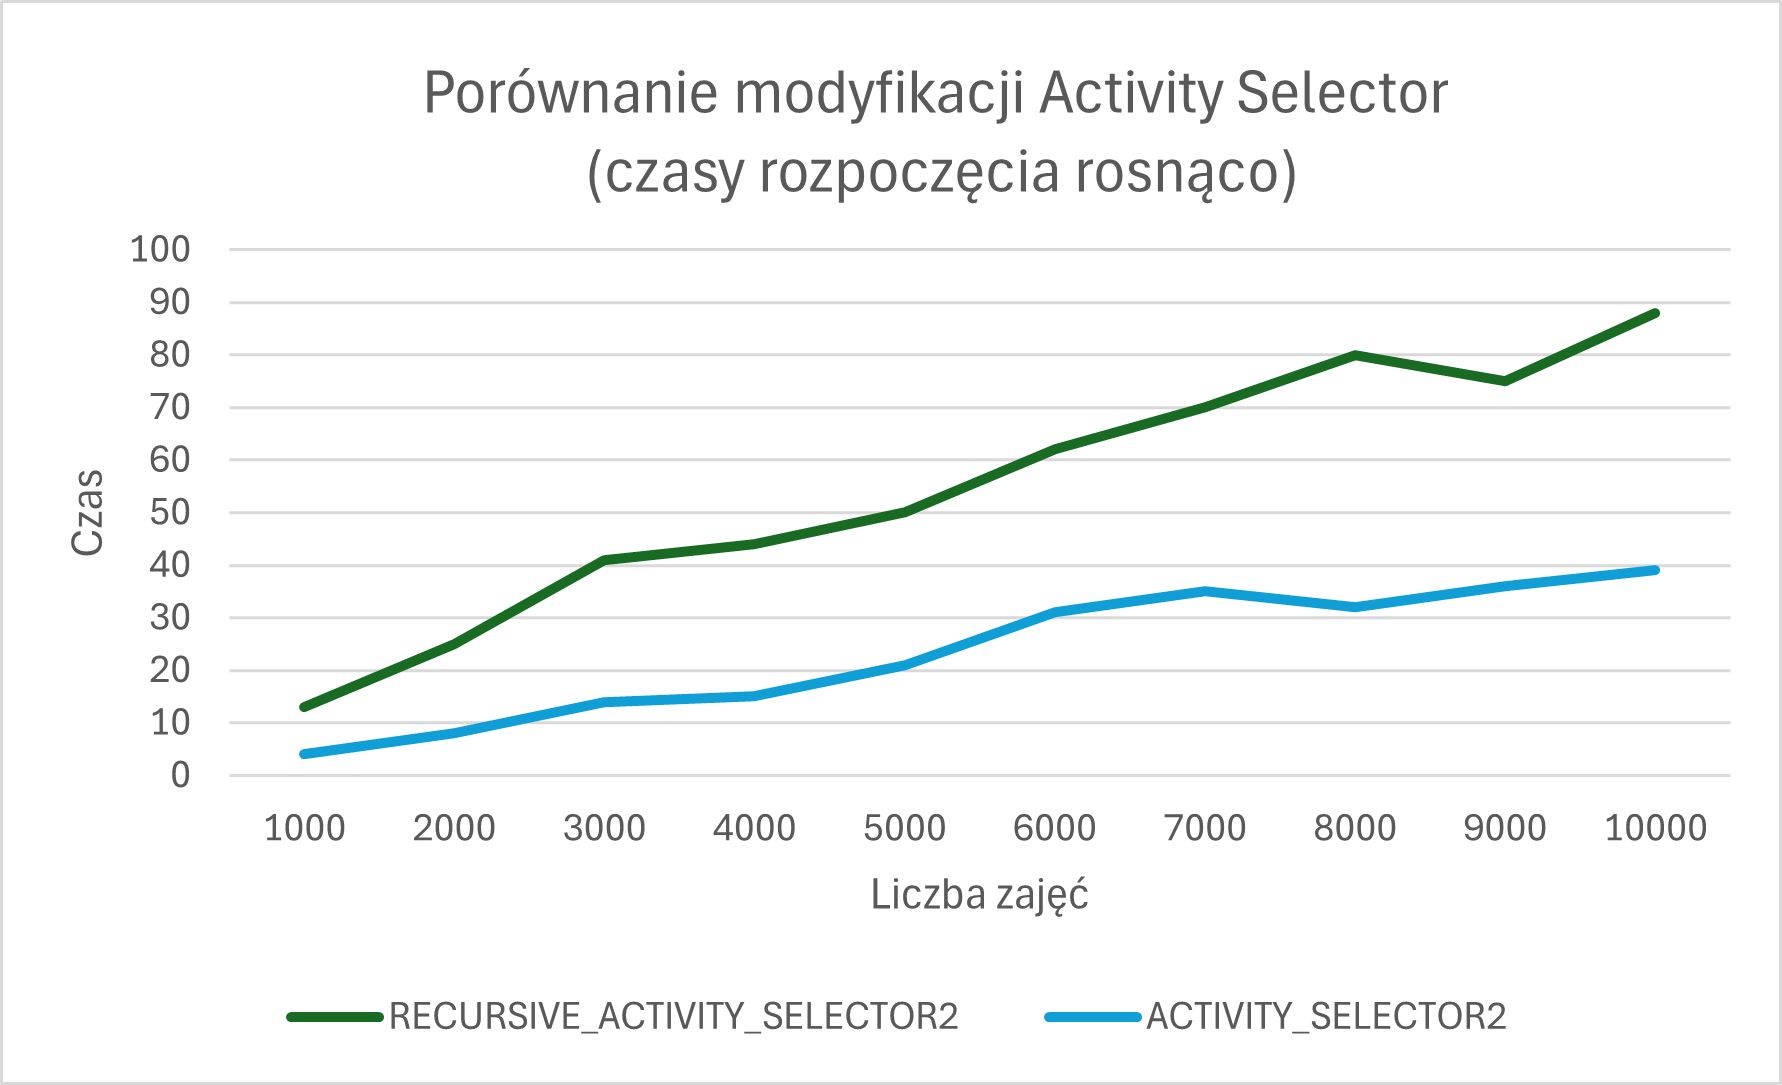
\includegraphics[width=\textwidth]{AS2.png}
		\end{minipage}
		\end{figure}
		
		\begin{figure}[H]
			\centering
			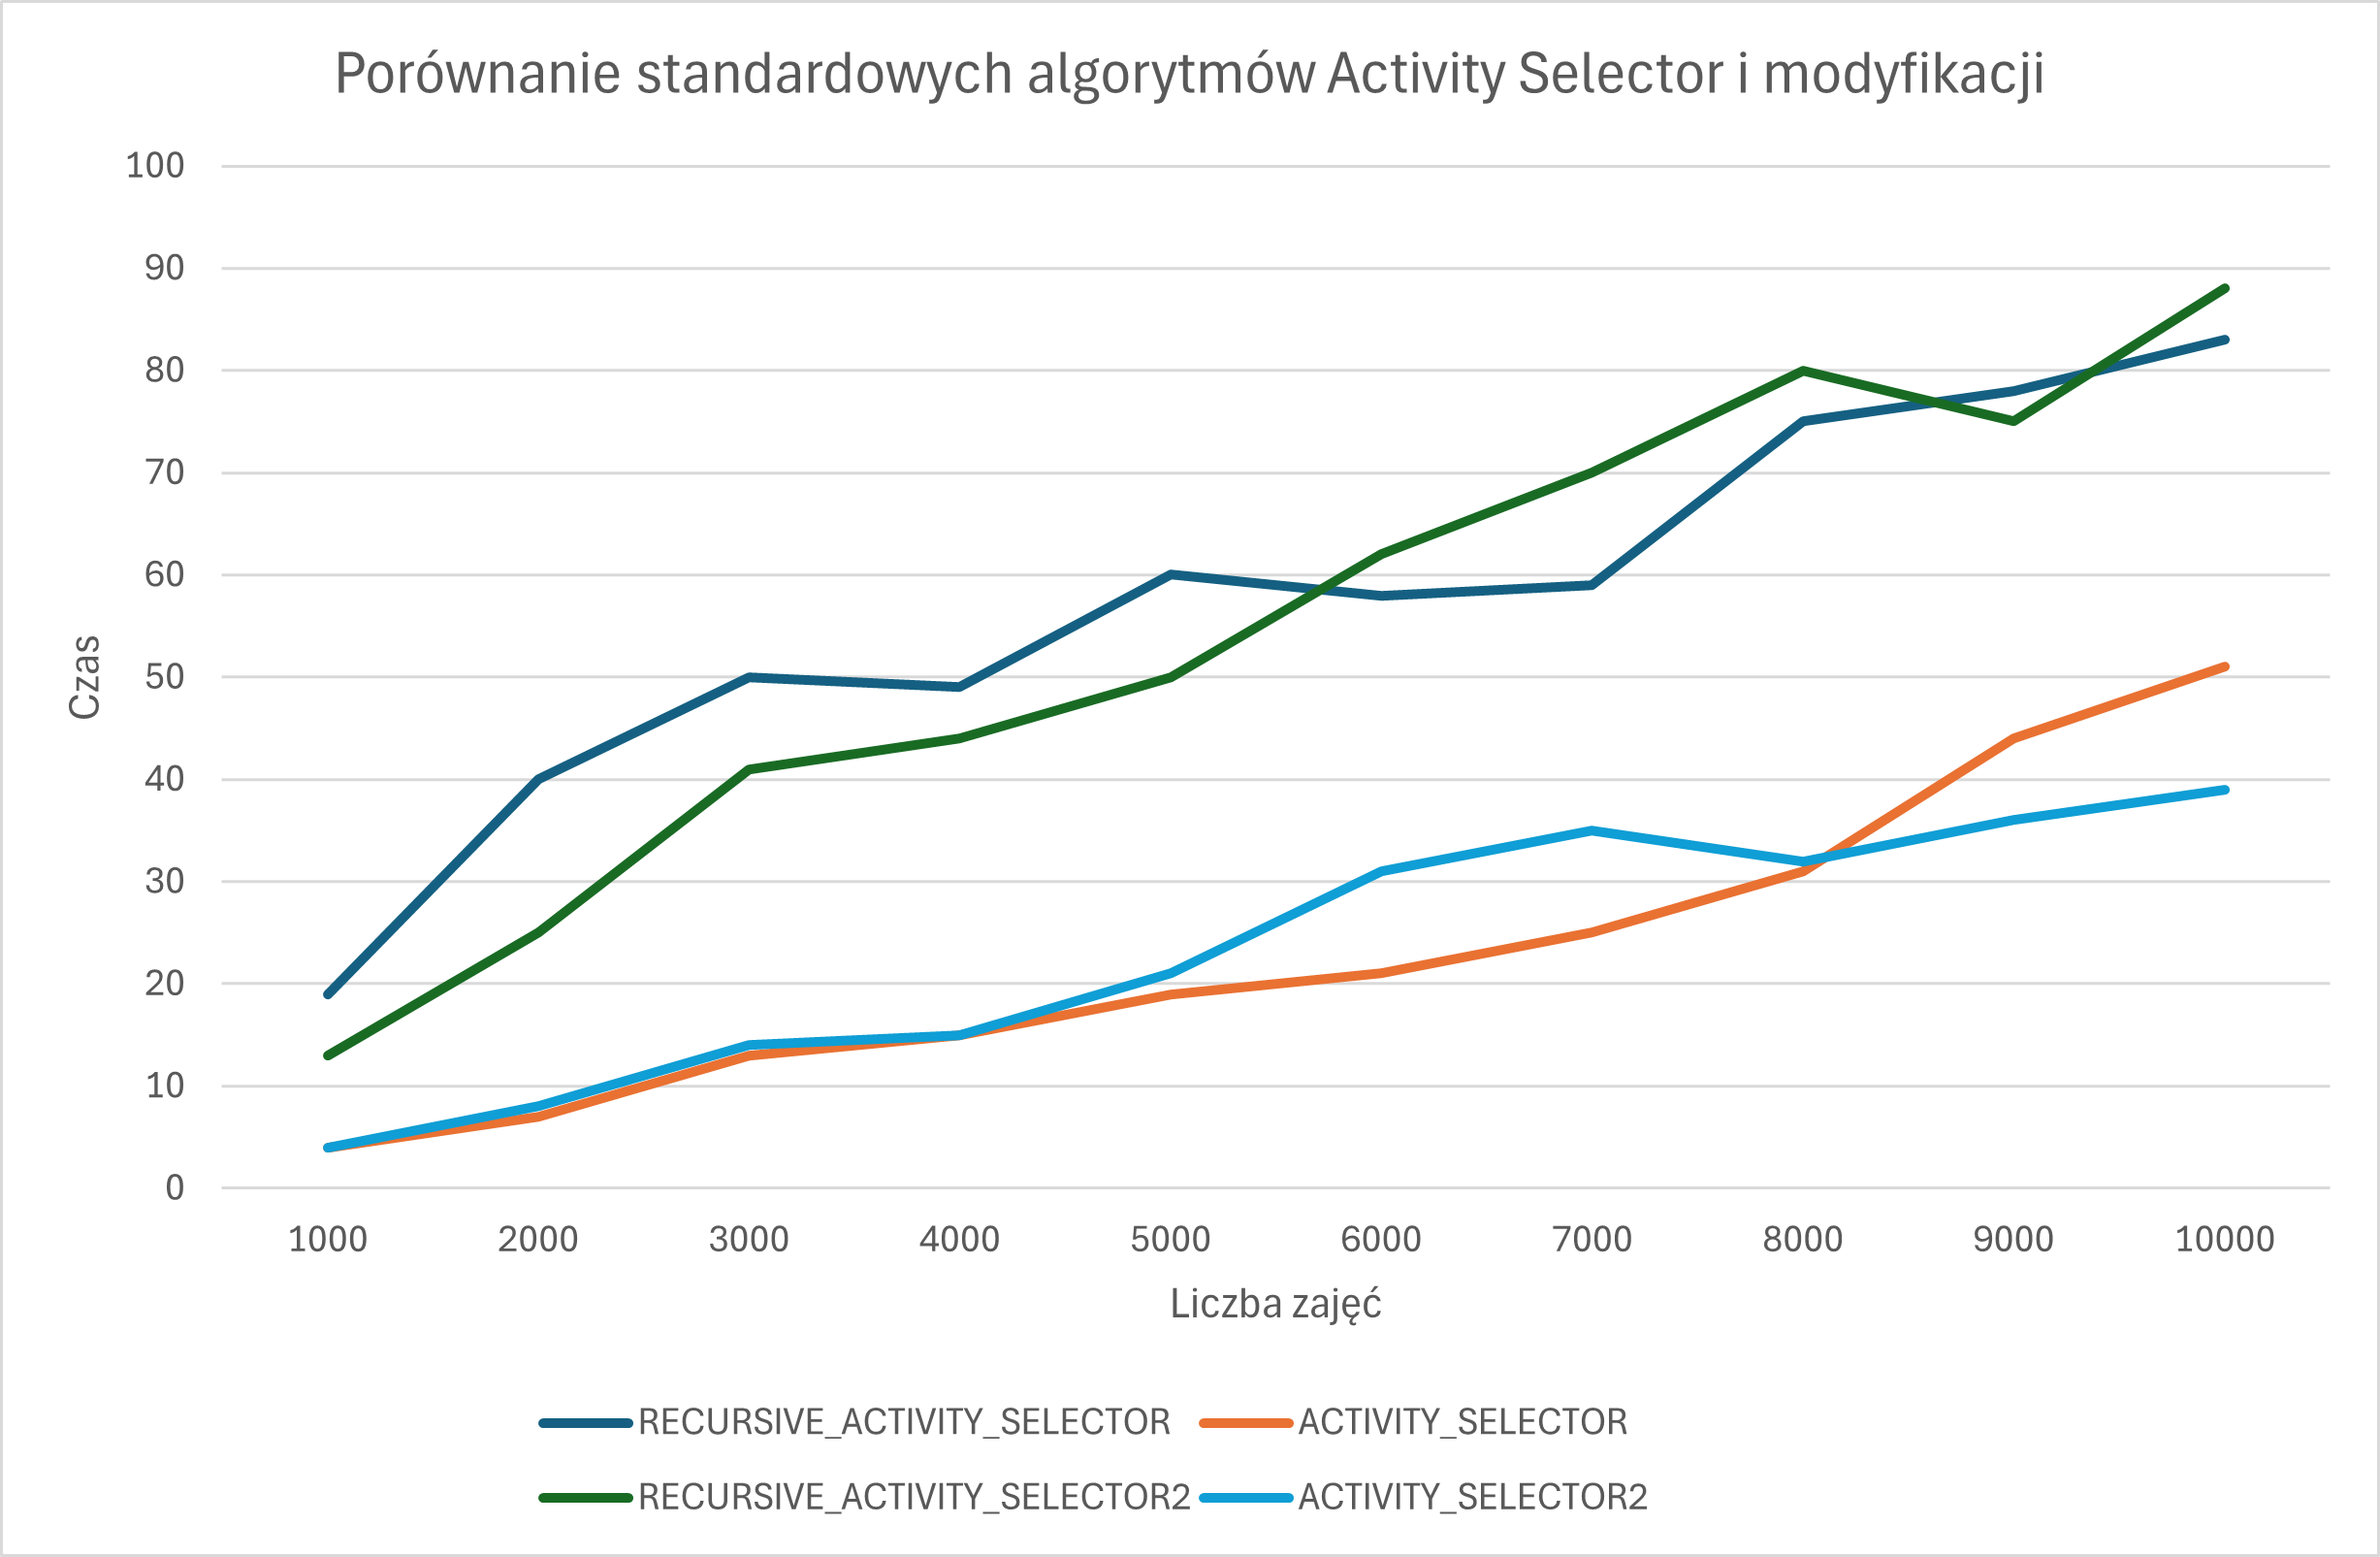
\includegraphics[width=0.9\textwidth]{PorAS.png}
		\end{figure}
		
		\subsection*{Wnioski} 
		Algorytm RECURSIVE\_ACTIVITY\_SELECTOR wykazuje wzrost czasu działania wraz ze wzrostem liczby zajęć. Rekurencja sprawia, że jest mniej efektywny przy dużych danych.
		Algorytm ACTIVITY\_SELECTOR, wykorzystuje podejście iteracyjne, z złożonością czasową $O(n)$. Jego wydajność pozostaje stosunkowo wysoka nawet dla dużej liczby zajęć. Algorytm RECURSIVE\_ACTIVITY\_SELECTOR2 na danych posortowanych względem czasu rozpoczęcia osiąga podobne wyniki do standardowej wersji, z lekkimi różnicami w czasie. Algorytm ACTIVITY\_SELECTOR2 dla danych posortowanych względem czasu rozpoczęcia również wykazuje bardzo podobne czasy działania jak standardowy ACTIVITY\_SELECTOR. To wskazuje, że sortowanie wejściowych danych względem czasu rozpoczęcia nie wpływa istotnie na jego efektywność. 
		
		\begin{figure}[H]
			\centering
			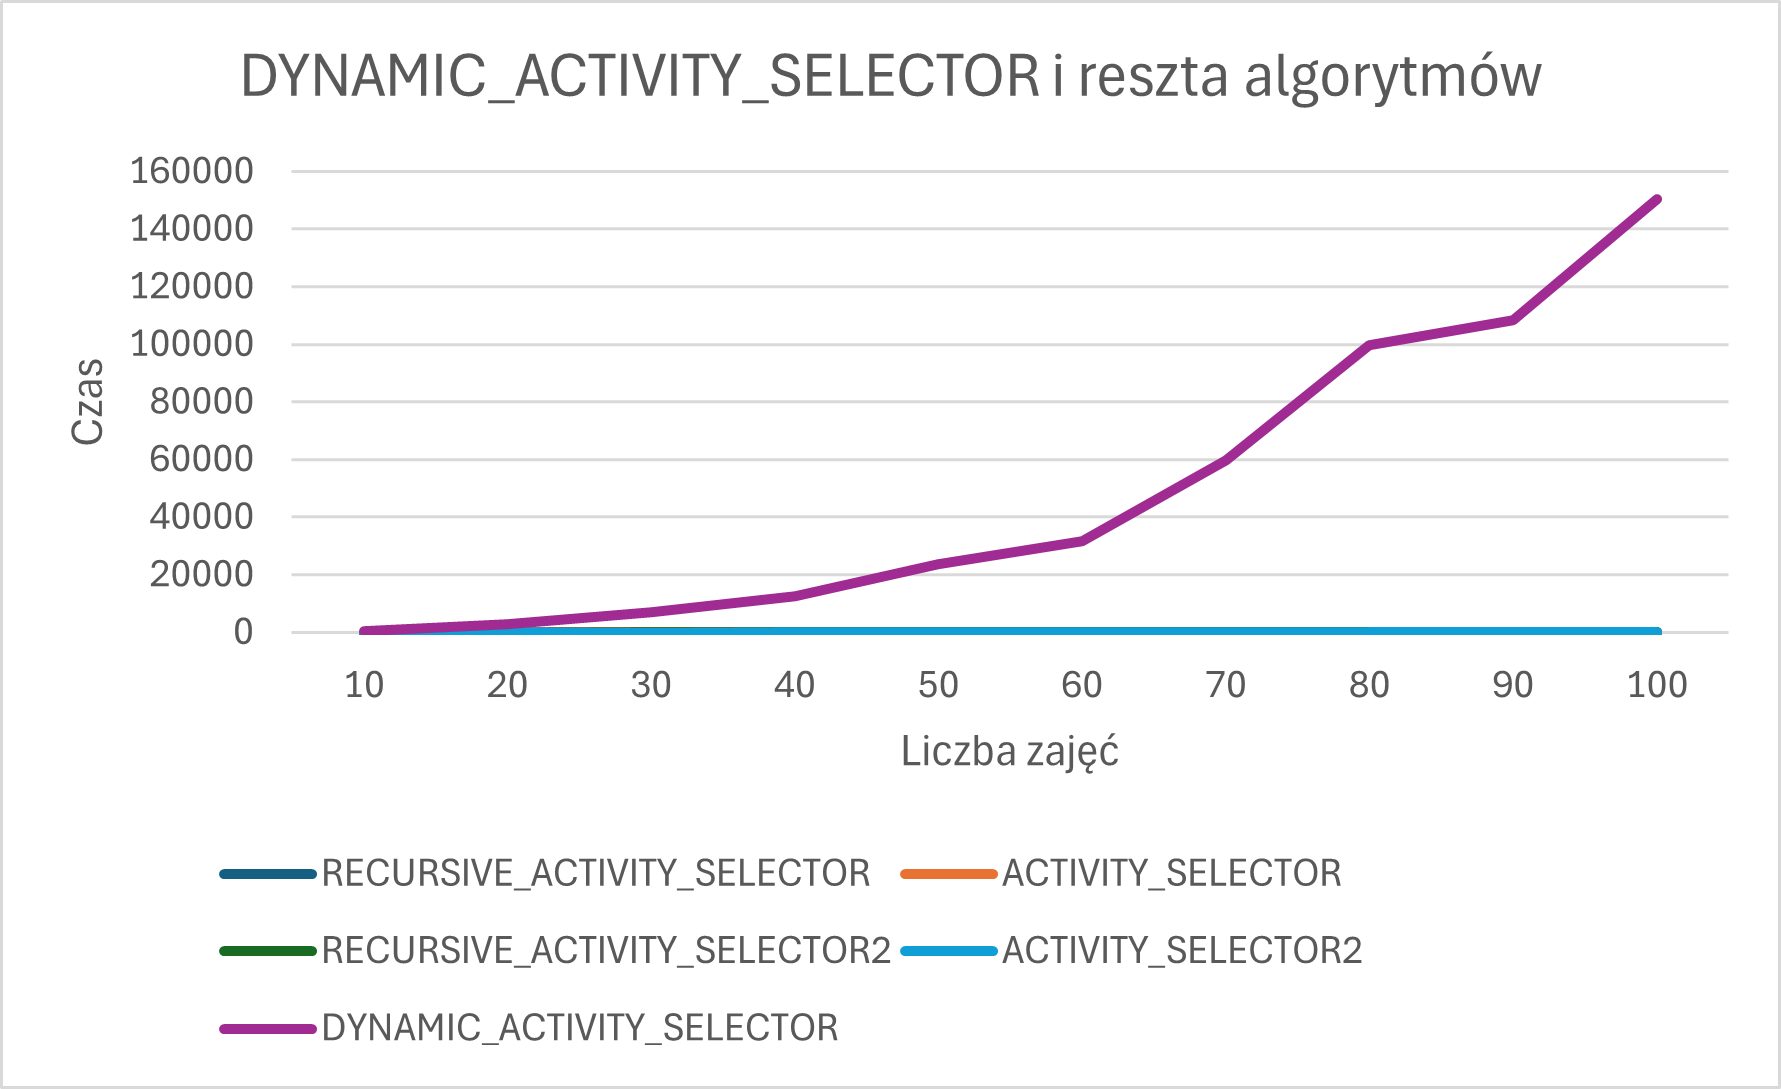
\includegraphics[width=0.9\textwidth]{DASiR.png}
		\end{figure}
		
		\subsection*{Wnioski} 
		Algorytm DYNAMIC\_ACTIVITY\_SELECTOR charakteryzuje się znacząco większym kosztem obliczeniowym w porównaniu do pozostałych, rosnącym gwałtownie wraz ze wzrostem liczby zajęć. Pozostałe algorytmy są znacznie bardziej wydajne, co czyni je praktyczniejszymi dla większych danych.

\end{document}